%%%%%%%%%%%%%%%%%%%%%%%%%%%%%%%%%%%%%%%%%
% Structured General Purpose Assignment
% LaTeX Template
%
% This template has been downloaded from:
% http://www.latextemplates.com
%
% Original author:
% Ted Pavlic (http://www.tedpavlic.com)
%
% Note:
% The \lipsum[#] commands throughout this template generate dummy text
% to fill the template out. These commands should all be removed when 
% writing assignment content.
%
%%%%%%%%%%%%%%%%%%%%%%%%%%%%%%%%%%%%%%%%%

%----------------------------------------------------------------------------------------
%	PACKAGES AND OTHER DOCUMENT CONFIGURATIONS
%----------------------------------------------------------------------------------------

\documentclass{article}[paper=a4,pagesize=auto,10pt]

\usepackage{fancyhdr} % Required for custom headers
\usepackage{extramarks} % Required for headers and footers
\usepackage{graphicx} % Required to insert images
\usepackage{algorithm2e}
\usepackage{amsmath}

\usepackage{booktabs}
\usepackage{floatrow}
% Table float box with bottom caption, box width adjusted to content
\newfloatcommand{capbtabbox}{table}[][\FBwidth]
\usepackage{subfig}
\usepackage{helvet}
\renewcommand{\familydefault}{\sfdefault}
\usepackage[T1]{fontenc}
%\usepackage{fontspec}
%\setmainfont{Arial}

% Margins
\topmargin=-0.45in
\evensidemargin=0in
\oddsidemargin=0in
\textwidth=6.5in
\textheight=9.0in
\headsep=0.25in 

\linespread{1.1} % Line spacing


%----------------------------------------------------------------------------------------
%	HEADER AND FOOTER
%----------------------------------------------------------------------------------------

% Set up the header and footer
\pagestyle{fancy}
\rhead{Albert Bezzina, Daniel Farrugia \& Ivan Salomone} % Top left header
\lhead{\hmwkClass\ - \hmwkTitle}

\lfoot{} % Bottom left footer
\cfoot{Page\ \thepage} % Bottom center footer
\rfoot{} % Bottom right footer
\renewcommand\headrulewidth{0.4pt} % Size of the header rule
\renewcommand\footrulewidth{0.4pt} % Size of the footer rule

\setlength\parindent{0pt} % Removes all indentation from paragraphs

   
%----------------------------------------------------------------------------------------
%	NAME AND CLASS SECTION
%----------------------------------------------------------------------------------------

\newcommand{\hmwkTitle}{Applied Machine Learning} % Assignment title
\newcommand{\hmwkClass}{ICS5110} % Course/class

%----------------------------------------------------------------------------------------
%	TITLE PAGE
%----------------------------------------------------------------------------------------

\title{
\textmd{\textbf{University of Malta}}\\

\includegraphics[width=3.5cm,height=5cm,keepaspectratio]{graphics/umlogo_red.png}\\
\vspace{2.0in}
\textmd{\textbf{\hmwkClass:\ \hmwkTitle}}\\
\vspace{0.1in}Bankruptcy prediction using Logistic Regression and Bagged Decision Trees\\
\vspace{2.0in}
}

\author{\textbf{Albert Bezzina (279484M)}, \textbf{Daniel Farrugia (384479M)} \& \textbf{Ivan Salomone (358379M)}}
%279484M, 384479M

\date{January 2019} % Insert date here if you want it to appear below your name

%----------------------------------------------------------------------------------------

\begin{document}

\maketitle
\thispagestyle{empty}
%----------------------------------------------------------------------------------------
%	TABLE OF CONTENTS
%----------------------------------------------------------------------------------------

%\setcounter{tocdepth}{1} % Uncomment this line if you don't want subsections listed in the ToC

\newpage
%\pagenumbering{roman}
\tableofcontents
\thispagestyle{empty}
\newpage
\pagenumbering{arabic}

%----------------------------------------------------------------------------------------
%	INTRODUCTION
%----------------------------------------------------------------------------------------

\section{Introduction}
\label{Introduction}

Companies having liquidity problems face what is know as \textit{financial distress}, that is the company’s operating cash flow is insufficient to meet its current liabilities \cite{tasman}. Financial distress forces companies to take unwanted measures, such as reducing the work force or downsizing operations, in order to alleviate the problem. Failing to emerge from financial distress leads a company to \textit{bankruptcy}, that is a situation where a company is unable to operate any longer due to its liquidity problems.\medskip

Bankruptcy affects the social community, business partners, investors, policy makers and the economy as a whole \cite{zikeba2016ensemble}. The high costs of bankruptcy led many researchers to seek means of anticipating it. Such studies date back to the 1930's when economists used financial indicators to predict business failures. Statistical models for bankruptcy prediction were introduced in the 1960's. Later in the 1990's, artificial intelligence and machine learning models took over.\medskip

In this assignment we demonstrate the use of \textit{Bagged Decision Trees} and \textit{Logistic Regression} models to predict companies going bankrupt based on their financial indicators. In doing so, we also discuss the steps taken to improve the predictive performance of the two models. Moreover, in Section 2 we give some theoretical background on the techniques that were used in this study. In Section 3 we describe the methods we used to pre-process the data, build and train the predictive models and finally evaluate the results. We also describe the experiments that were conducted on the inferred models. To conclude, in Section 4 we discuss the findings of this study.

\subsection{The Dataset} \label{The Dataset}

The dataset that is used for this assignment was created by Zikerba et al. \cite{zikeba2016ensemble} in a study aimed at demonstrating bankruptcy prediction through an ensemble of boosted trees. It consists of five years of Polish company financial indicators, together with a class indicating whether the company goes bankrupt in the sixth year.  Therefore, for \textit{Year~1} the class indicates whether the company goes bankrupt in $t+5$ years (1=bankrupt, 0=solvent) whilst for \textit{Year~5} the class refers to $t+1$ year. The data for each year resides in a separate ARFF\footnote{Attribute-Relation File Format} file. The attributes, 64 in total, consist of accounting ratios such as \textit{net profit / total assets} and \textit{total liabilities / total assets}. A description of all the attributes can be found in the dataset description page\footnote{http://archive.ics.uci.edu/ml/datasets/Polish+companies+bankruptcy+data}.\medskip

\begin{table}[ht]
\centering
\begin{tabular}{lrrrrr}
\toprule
Year            &     1 &      2 &      3 &     4 &     5 \\
\midrule
\# samples      &  7027 &  10173 &  10503 &  9792 &  5910 \\
\addlinespace[0.2cm]
\% bankrupt     &     4 &      4 &      5 &     5 &     7 \\
\% solvent      &    96 &     96 &     95 &    95 &    93 \\
\addlinespace[0.2cm]
\% correlated   &    10 &     10 &     6 &    8 &    10 \\
\% uncorrelated &    90 &     90 &     94 &    92 &    90 \\
\addlinespace[0.2cm]
\% missing      &     1 &      2 &      1 &     1 &     1 \\
\% outliers     &     1 &      1 &      1 &     1 &     1 \\

\bottomrule
\end{tabular}
\caption{The percentages of bankrupt/solvent companies as an indication of imbalance, correlation between attributes, and the percentage of missing values and outliers, across the various years.}
\label{tab:dataset}
\end{table}

The results of a preliminary study of the data are presented in Table \ref{tab:dataset}. A considerable imbalance in the class can be noted, given that the majority of companies are solvent in the sixth year. This is important to note due to its negative impact on the machine learning process. Other aspects that impair the classification ability of the models are missing values and outliers. Although the percentage of missing values and outliers is relatively small, proper handling of these is likely to give better results. \medskip

It was also found that some of the attributes are closely correlated. This is not surprising because some of the accounting ratios are closely tied. For example a correlation coefficient of 1 was found between \textit{EBIT\footnote{Earnings Before Interest and Taxes} / total assets}, \textit{(gross profit + interest) / total assets} and \textit{gross profit / total assets}. Table \ref{tab:dataset} shows the percentage of pairwise attributes that have a \textit{correlation coefficient} ($r$) $\geq$ 0.5. Figure~\ref{fig:heatmap} shows a correlation heatmap for the dataset of \textit{Year 1}.

\begin{figure}[!ht]
    \centering
    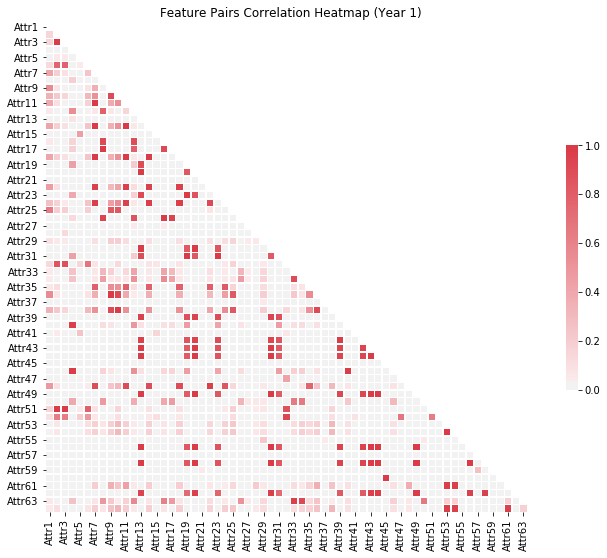
\includegraphics[width=0.7\textwidth]{graphics/heatmap_year1.png}
    \caption{A correlation heatmap for Year 1.}        
    \label{fig:heatmap}
\end{figure}




%----------------------------------------------------------------------------------------
%	BACKGROUND
%----------------------------------------------------------------------------------------

\section{Background}
\label{Background}

\subsection{Logistic Regression} \label{Logistic Regression}

Logistic regression is a probabilistic discriminative model \cite{bishop2006}.  It is a binary classifier that models the probability that an instance belongs to either of two classes (i.e. 1 or 0, True or False, etc.) \cite{james2013introduction}.  For each instance \textit{i} the model will produce a probability that \textit{i} belongs to a class \textit{c\textsubscript{0}} (i.e. $Pr(Y\textsubscript{i} = c\textsubscript{0}|x\textsubscript{i})$).  Then the model will classify \textit{i} as \textit{c\textsubscript{0}} if the probability is greater than a particular threshold.  In many cases the threshold is set to 0.5, but this varies according to the problem at hand. \medskip

This is done by using the techniques from linear regression shown in Equation \ref{eq:logistic1}, where \textit{x\textsubscript{1i}} to \textit{x\textsubscript{ni}} are the values of the various attributes of instance \textit{i}, $\beta\textsubscript{0}$ to $\beta\textsubscript{n}$ are the corresponding weights associated to each attribute \cite{sammut2017encyclopedia}.

\begin{equation}\label{eq:logistic1}
	z\textsubscript{i} = \beta\textsubscript{0} + \beta\textsubscript{1}x\textsubscript{1i} + \beta\textsubscript{2}x\textsubscript{2i} + ... + \beta\textsubscript{n}x\textsubscript{ni}
\end{equation}\smallskip

Given that this does not produce a probability between 0 and 1 as required for binary classification, the resulting \textit{z\textsubscript{i}} is plugged into the logistic (or sigmoid) function (Equation \ref{eq:logistic2}) to produce the desired result \cite{sammut2017encyclopedia}.  This is shown in Figure \ref{fig:logistic_graph} where the plot (a) shows the estimated probability of default using the linear equation (Equation \ref{eq:logistic1}) while the plot (b) shows the probability transformed through the logistic function (Equation \ref{eq:logistic2}) \cite{james2013introduction}. Although Figure~\ref{fig:logistic_graph} shows plots for univariate data, logistic regression can also be performed on multivariate datasets.

\begin{equation}\label{eq:logistic2}
	Pr(c\textsubscript{0}|x\textsubscript{1i}...x\textsubscript{ni}) = \frac{1}{1 + e^{-z\textsubscript{i}}}
\end{equation}\smallskip

The weight coefficients $\beta\textsubscript{0}$ to $\beta\textsubscript{n}$ are estimated upon the training data and are determined by the maximum likelihood estimation \cite{james2013introduction,dreiseitl2002logistic}. In other words, the vector $\alpha$ of parameters $\beta\textsubscript{0}$ to $\beta\textsubscript{n}$ is chosen so as to maximise $\prod_{i=1}^{n}\ Pr(y\textsubscript{i}|x\textsubscript{i},\alpha)$. This can be achieved using using various methods amongst which gradient descent \cite{dreiseitl2002logistic}.\medskip

\begin{figure}[!ht]
    \centering
    \subfloat[A plot using the linear function.]{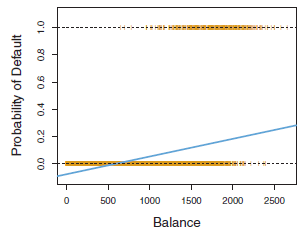
\includegraphics[width=0.45\textwidth]{graphics/logistic_a.png}}\qquad
    \subfloat[The predicted probabilities transformed using the logistic function.]{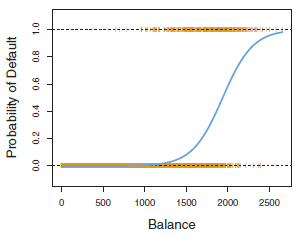
\includegraphics[width=0.45\textwidth]{graphics/logistic_b.png}}%
    \caption[Short Caption]{A plot of the \textit{Probability of Default} against the \textit{Balance} \cite{james2013introduction}.}        
    \label{fig:logistic_graph}
\end{figure}

Although inherently a binary classifier, logistic regression can be extended to classify more than two classes \cite{allwein2000reducing}. The approach involves simplifying the multiclass problem into a number of binary problems, whereby for every class, a logistic regression classifier is trained to determine whether an instance is a member of the class or not.  The multiclass classification is achieved by evaluating the output of the various classifiers to establish the class.  This is known as the one-against-all approach.\medskip

Logistic regression is found to be less prone to overfitting than other models \cite{dreiseitl2002logistic}. However, it is intolerant to noise and outliers.

\subsection{Bagged Decision Trees} \label{Bagged Decision Trees}

\subsubsection{Decision Trees} \label{Decision Trees}

A decision tree is a classifier that takes the form of nodes and branches \cite{han2011data}. Internal nodes represent a test on some feature, while the branches represent the outcomes of the test, leading to another internal node or a leaf node. Each leaf node represents a class. The topmost node is called the root node. Decision trees can deal with both \textit{discrete-valued} and \textit{continuous-valued} attributes. Continuous values are expressed as conditions by introducing \textit{split-points}, for example $salary<10,000$ and $salary\geq10,000$.  \medskip

Decision tree induction algorithms include ID3, C4.5 and CART, which adopt a greedy approach (i.e. without backtracking) to the tree construction \cite{han2011data}. The tree is built recursively top-down, starting from the root node \cite{sammut2017encyclopedia,han2011data}. The algorithms place at the root the attribute that best discriminates the training data. For example, let \textit{D} be the sample dataset shown in Table \ref{tab:dt_data}. The algorithm evaluates the four attributes (note that \textit{Play Golf} is the class) and it results that \textit{outlook} best discriminates the data. So \textit{outlook} is placed at the root. Next, the possible outcomes of \textit{outlook} are set as branches. For each branch, the dataset is partitioned by the respective outcome. If all the examples in the partitioned dataset are of the same class then a leaf node is added and set to this class. It can be noted that for \textit{D\textsubscript{overcast}} this holds, so a leaf node with class \textit{yes} is added. But not for \textit{D\textsubscript{sunny}} so once again the attribute that best discriminates \textit{D\textsubscript{sunny}} is set as the node. The algorithm iterates until all leaf nodes are filled. Figure \ref{fig:decision_tree} shows the resulting tree. \medskip

\begin{equation}\label{eq:entropy}
	Entropy(S) = \sum_{i=1}^{c} -p\textsubscript{i} log\textsubscript{2}p\textsubscript{i}
\end{equation}\smallskip

\begin{equation}\label{eq:gain}
	Gain(S,A) =  Entropy(S) - \sum_{v\in values(A)} \frac{|S\textsubscript{v}|}{S} Entropy(S)
\end{equation}\smallskip

The function used to measure how much an attribute discriminates the data varies according to the algorithm being used \cite{han2011data}. ID3 uses \textit{information gain} while C4.5 uses \textit{gain ratio}, that is a normalised form of the \textit{information gain}. CART on the other hand uses the \textit{Gini index}. The information gain is obtained through Equation~\ref{eq:gain}, where $Gain(S,A)$ is the information gain of an attribute $A$ relative to a collection of examples $S$, $values(A)$ are all the possible values of $A$, $S\textsubscript{v}$ is the subset of $S$ having $A=v$ and $Entropy(S)$ is obtained through Equation~\ref{eq:entropy}, where in turn $p\textsubscript{i}$ is the subset of $S$ belonging to class $i$.

\begin{figure}
\begin{floatrow}
\ffigbox{%
  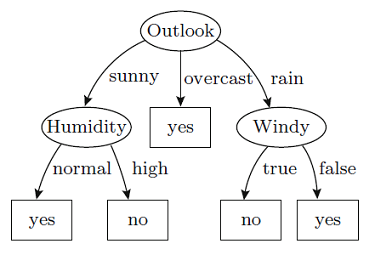
\includegraphics{graphics/decision_tree.png}%
}{%
  \caption{The resulting decision tree after training on the data in Table \ref{tab:dt_data} \cite{sammut2017encyclopedia}.}
  \label{fig:decision_tree}%
}
\capbtabbox{%
  \begin{tabular}{lllll}
\toprule
Outlook & Temp & Humidity & Windy & Play Golf \\
\midrule
rainy & hot & high & false & no \\
rainy & hot & high & true & no \\
overcast & hot & high & false & yes \\
sunny & mild & high & false & yes \\
sunny & cool & normal & false & yes \\
sunny & cool & normal & true & no \\
overcast & cool & normal & true & yes \\
rainy & mild & high & false & no \\
rainy & cool & normal & false & yes \\
sunny & mild & normal & false & yes \\
rainy & mild & normal & true & yes \\
overcast & mild & high & true & yes \\
overcast & hot & normal & false & yes \\
sunny & mild & high & true & no
%\bottomrule
\end{tabular}
}{%
  \caption{A sample dataset adapted from \cite{sammut2017encyclopedia}.}
  \label{tab:dt_data}%
}
\end{floatrow}
\end{figure}

\subsubsection{Tree Pruning} \label{Tree Pruning}

Decision tree induction is prone to \textit{overfitting}, especially in the presence of noise or outliers \cite{han2011data}. Tree pruning is a method whereby part of a tree is removed to simplify or generalise the decision tree, thus addressing overfitting. Most commonly, a \textit{post-pruning} approach is used that prunes sub-trees from the induced tree. A sub-tree at a given node is removed and replaced by a leaf node, which is labelled with the class that featured most in the pruned sub-tree. Similarly, in \textit{pre-pruning} the tree construction process is stopped prematurely resulting in an unfinished decision tree.

\subsubsection{Bagging} \label{Bagging}

In bagging, \textit{n} classifiers are trained on \textit{n} random samples of the training data, taken with replacement \cite{quinlan1996bagging}. This results in \textit{n} different models. Classification of unseen instances is then done through a vote of all \textit{n} classifiers. Ties are decided arbitrarily. Experiments in \cite{quinlan1996bagging} show that \textit{bagged} decision trees outperform ordinary decision trees.

\subsection{Rescaling and Normalisation} \label{Rescaling and Normalisation}

Typically, features in a dataset have different scales and ranges, possibly incorporating very large numbers.  These discrepancies across features tend to hinder the performance of a learning algorithm \cite{han2011data}. Larger numbers give the feature a greater weight, thus giving it prominence over other possibly more important features that are of a smaller dimension.  This happens particularly in algorithms that use distance measurements such as \textit{k-nearest neighbour}, \textit{neural networks} and \textit{clustering}.  To overcome this, features are normalised or rescaled.  This involves transforming the values of the various features to a smaller range, such as between \textit{0} and \textit{1} \cite{han2011data,mohamad2013standardization,garcia2015data}. In literature, the terms normalisation and rescaling are used interchangeably.

\subsubsection{Min-max normalisation} \label{Min-max normalisation}

Min-max normalisation transforms the features to a range between \textit{0} and \textit{1} \cite{mohamad2013standardization}. The normalised value \textit{v}$'$ is obtained through Equation \ref{eq:minmax} where \textit{v} is the original unnormalised value, and \textit{A\textsubscript{min}} and \textit{A\textsubscript{max}} are respectively the minimum and maximum values of feature \textit{A}.

\begin{equation}\label{eq:minmax}
	v' = \frac{v - A\textsubscript{min}}{A\textsubscript{max}-A\textsubscript{min}}
\end{equation}\smallskip

\subsubsection{Z-score normalisation} \label{Z-score normalisation}

Z-score normalisation (sometimes referred to as \textit{standardisation}) transforms the data such that they have a mean of \textit{0} and a standard deviation of \textit{1} \cite{mohamad2013standardization,garcia2015data}. This is obtained through Equation \ref{eq:zscore} where value \textit{v} is transformed into a normalised value \textit{v}$'$. $\bar{A}$ is the mean of feature \textit{A} and $\sigma\textsubscript{A}$ is the standard deviation of \textit{A}.  

\begin{equation}\label{eq:zscore}
	v' = \frac{v - \bar{A}}{\sigma\textsubscript{A}}
\end{equation}\smallskip

This technique is particularly useful when the minimum and maximum of a feature are not known or when the data contain outliers \cite{garcia2015data}. In this technique a normal distribution is assumed \cite{stolcke2008nonparametric}.\medskip

\subsubsection{Decimal scaling} \label{Decimal scaling}

Decimal scaling divides all values of a feature by a common denominator so that all new normalised values \textit{v}$'$ fall in the range \textit{0 < v}$'$\textit{ < 1} \cite{han2011data,garcia2015data}.  This is achieved through Equation \ref{eq:decimal_scaling} where \textit{v} is the unnormalised value and \textit{j} is the smallest integer such that \textit{max(v}$'$\textit{) < 1}.

\begin{equation}\label{eq:decimal_scaling}
	v' = \frac{v}{10^j}
\end{equation}

\subsubsection{Quantile normalisation} \label{Quantile normalisation}

In quantile normalisation, the distribution of each feature is harmonised \cite{bolstad2003comparison}.  To normalise a dataset \textit{X} made up of \textit{n} instances having \textit{p} attributes, the values making up each instance are first sorted to make up \textit{X\textsubscript{sort}}. It should be noted that the dimensions of \textit{X\textsubscript{sort}} are not the same attributes of \textit{X} since these are now mixed-up through sorting. \textit{X}$'$\textit{\textsubscript{sort}} is then created by changing the value of each element within every dimension of \textit{X\textsubscript{sort}} to the mean of its respective dimension. The normalised dataset \textit{X}$'$ can then be acquired by reordering the instances of \textit{X}$'$\textit{\textsubscript{sort}} to the original order of \textit{X}.  This normalisation method is very robust to outliers since the extreme values are replaced by the means.

\subsubsection{Normalisation parameters} \label{Normalising parameters}

When normalising data, it is imperative that the normalisation parameters used to transform the data (eg. the \textit{mean} and \textit{standard deviation} in \textit{z-score normalisation} or \textit{j} in \textit{decimal scaling}) are saved for later use \cite{han2011data}. When new instances need to be classified these have to be normalised using these same parameters.

\subsection{Cross-validation} \label{Cross-validation}

The error rate of a learning function should be estimated upon unseen observations since the performance of the function varies considerably upon seen and unseen instances \cite{james2013introduction}. Therefore, a subset of observations is held-out from the training set upon which the model is fit and then used to estimate the error rate. This subset is referred to as the test (or validation) set. Cross-validation (CV) extends upon this method by averaging the error rate of several hold-out runs using different data splits \cite{arlot2010survey}.

CV techniques can be categorised as \textit{exhaustive data splitting} approaches and \textit{partial data splitting approaches} \cite{arlot2010survey}.

\subsubsection{Exhaustive data splitting CV} \label{Exhaustive data splitting CV}

In exhaustive data splitting, the size \textit{n\textsubscript{t}} of the training set is decided in advance, and all possible training sets of size \textit{n\textsubscript{t}} are considered, i.e. all possible combinations of splitting the training data into a training set of size \textit{n\textsubscript{t}} are eventually used for training and evaluation \cite{arlot2010survey}. \textit{Leave-one-out} is one such method where \textit{n\textsubscript{t}} is taken as \textit{n-1}. All possible training sets are used, each time holding out one observation that is then used for testing.  \textit{Leave-p-out} adopts the same approach but in this case \textit{n\textsubscript{t}} is taken as \textit{n-p}.

\subsubsection{Partial data splitting CV} \label{Partial data splitting CV}

In \textit{k-fold} (or \textit{v-fold}) CV, the error rate is estimated over \textit{k} iterations of training \cite{arlot2010survey}. The training data is randomly split into \textit{k} segments, each of which is taken as a test set for one of the iterations. In some cases, the folds are stratified to contain approximately the same number of instances from each class thus keeping the dataset balanced \cite{kohavi2001}.  Experiments carried out by \cite{kohavi2001} suggest the use of ten or more folds ($k\geq10$) since the bias is reduced considerably. \medskip

\textit{Balanced incomplete} CV is another technique where test sets are systematically chosen in such a way to maintain a balance between the various data points \cite{shao1993linear}. Specifically, the test sets are chosen in such a way that every data point appears in the same number of test sets, and every pair of instances appear in the same number of test sets. \medskip

\textit{Monte-Carlo CV} and \textit{repeated learning-testing CV} are another two partial data splitting approaches that are very similar \cite{arlot2010survey}. Both approaches consider several test sets of size \textit{n\textsubscript{v}} that are chosen at random. The difference between the two approaches is that in Monte-Carlo CV the test sets are generated with replacement while in repeated learning-testing CV the test sets are generated without replacement.

\begin{figure}[ht]
  	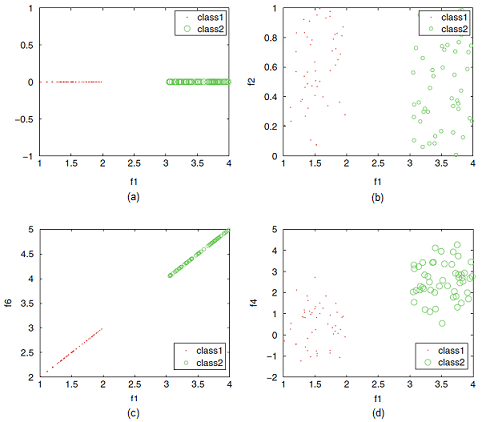
\includegraphics{graphics/feature_selection3.png}
  	\caption{Example plots showing (a) a relevant feature, (b) an irrelevant feature, (c) a redundant feature and (d) a noisy feature \cite{sammut2017encyclopedia}.}
  	\label{fig:feature_selection}
\end{figure}

\subsection{Feature Selection and Dimensionality Reduction Methods} \label{Feature Selection and Dimensionality Reduction Methods}

Having many features introduces a number of challenges to machine learning.  Not all features may be relevant to the problem and these confuse the learner resulting in a decrease in the predicting capability \cite{sammut2017encyclopedia}.  Moreover, having many features requires more training time and more computation capacity \cite{guyon2003introduction}. There is also an increased risk of overfitting \cite{de2015feature}.  Therefore in the pre-processing phase we aim to reduce the number of dimensions whilst keeping the information that is important to the learning process.




\subsubsection{Feature selection} \label{Feature selection}

To reduce the number of dimensions that are used for learning, feature selection retains a subset of the dimensions that are related to the class label whilst the remaining dimensions are discarded [intro].  A dimension is discarded if it is found to be irrelevant, redundant or noisy \cite{sammut2017encyclopedia}.  For example, considering feature \textit{f1} as shown in Figure \ref{fig:feature_selection}a, it can be seen that \textit{f1} is a relevant feature because it can distinguish between the classes. Feature \textit{f2} (Figure \ref{fig:feature_selection}b) on the other hand is unable to distinguish between the two classes and is therefore irrelevant for the classification and hence discarded.  As seen in Figure \ref{fig:feature_selection}c, feature \textit{f6} is also a relevant feature because it perfectly distinguishes between the two classes.  However, f6 does not add any new information that \textit{f1} has not already provided, so it is said to be a redundant feature. Feature \textit{f4} (Figure \ref{fig:feature_selection}d) is partly able to distinguish between the two classes.  The overlapping instances are either caused by errors in the data (noise) or due to the nature of the attribute.  This type of feature is said to be noisy and is also discarded. There are three models used for feature selection: filter, wrapper and embedded.

\paragraph{Filter models -}

Filter models rank the features by their relevance to the problem or by the degree of new information that is added \cite{de2015feature}.  \textit{Mutual information}, \textit{Pearson’s correlation} and \textit{maximum-relevance-minimal-redundancy} are commonly used as score functions upon which to rank the features \cite{de2015feature}. Once the features are ranked, the top-ranking features are chosen whilst the others are discarded \cite{sammut2017encyclopedia}.

\paragraph{Wrapper models -}

The filter models discussed above consider features individually assuming them independent, which may or may not be true.  Low ranked features may still contribute towards a prediction when considered together with other features \cite{de2015feature}. Wrapper models address this limitation by evaluating subsets of features rather than individual features. Figure \ref{fig:wrapper} shows a conceptual view of a wrapper model.  The \textit{subset generation} component takes on the original features and uses a search strategy to generate subsets of features for evaluation.  The \textit{subset evaluation} component utilises the learning algorithm upon the subset to measure and evaluate its performance.  These steps are repeated until a \textit{stopping criterion} is met.  Typically, the stopping criterion is that refinements to the subset do not yield any performance improvements. Another improvement on the Filter model is that since the learning algorithm is involved in the selection of the subset, any bias introduced by the chosen algorithm is removed \cite{sammut2017encyclopedia}.  The drawback of this model is that, while Filter models are very efficient, wrapper models are very computationally expensive.


\begin{figure}[ht]
  	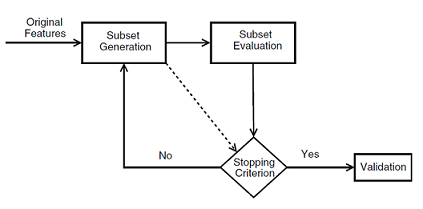
\includegraphics{graphics/wrapper.png}
  	\centering
  	\caption{A conceptual view of a Wrapper Model \cite{de2015feature}.}
  	\label{fig:wrapper}
\end{figure}



\paragraph{Embedded models -}

Some learning algorithms have in-built mechanisms to deal with feature selection \cite{guyon2003introduction,sammut2017encyclopedia}. This makes the selection of the features more efficient than the wrapper method and is specifically designed for the algorithm of choice. Another improvement on the other methods is that whilst the filter and wrapper methods select the features as part of the pre-processing of the data, the embedded models cater for feature selection as part of the learning process. One such example is the use of \textit{l1-norm} regularisation in \textit{Support Vector Machines} (SVM) \cite{guyon2003introduction,de2015feature}. Here the coefficients of less important features are reduced to zeros thus eliminating them. \textit{L2-norm} regularisation can also be used for feature selection but was found to be less effective than \textit{l1-norm} regularisation \cite{de2015feature}. \textit{Decision trees} also have a feature selection strategy embedded within the algorithm \cite{garcia2015data}.

\subsubsection{Dimensionality reduction} \label{Dimensionality reduction}

In dimensionality reduction (or \textit{feature extraction}) the number of features is reduced by defining new dimensions that are smaller in number but can represent the original dimensions through a function \cite{garcia2015data,sammut2017encyclopedia}. In other words, a high-dimensional feature space is projected into a feature space having less dimensions. The challenge of dimensionality reduction is finding a feature space that preserves the information provided by the original dimensions \cite{sammut2017encyclopedia}.

\paragraph{Principal component analysis -}

Principal component analysis (PCA) searches for a set of linear transformations of the original dimensions that preserve the most variance and result in less dimensions \cite{garcia2015data}. The result is a number of n-dimensional orthogonal vectors. The dimension that contributes to the most variance of the original data is called the \textit{first principal component}. Generally not all principal components are kept but only those that are accountable for approximately 95\% of the variance.

\paragraph{Factor analysis -}

Factor analysis follows the same concept of PCA but instead of searching for transformations of the original dimensions, it looks for hidden factors among the dimensions \cite{garcia2015data}.

\paragraph{Multidimensional scaling -}

Multidimensional scaling looks at the distance between data points in a way to preserve the relationship between the data points \cite{garcia2015data}. After calculating the distance matrix, the dimensions of the data are no longer important since the structure is rebuilt through the distance matrix.

\paragraph{Local Linear Embedding -}

Local Linear Embedding builds on the assumption that for a non-linear manifold, the surface is linear at infinitesimal distance \cite{garcia2015data}. Dimensionality reduction is done by first finding the k-NN of each data point, then calculating the linear weights of the distances between the data points and their neighbours so that it can be mapped on a lower dimensional space.

\subsection{Quantitative Measurements for Model Evaluation} \label{Quantitative Measurements for Model Evaluation}

\subsubsection{Sensitivity and Specificity} \label{Sensitivity and Specificity}

Sensitivity (or \textit{true positive rate}) is the fraction of positive examples that are correctly labelled by a classification model \cite{sammut2017encyclopedia}. Specificity (or \textit{true negative rate}) on the other hand is the fraction of negative examples that are correctly labelled by a classification model \cite{sammut2017encyclopedia}. These measures are good candidates for evaluating \textit{class-imbalanced} datasets \cite{han2011data}. Sensitivity and specificity are calculated by Equation \ref{eq:sensitivity} and Equation \ref{eq:specitivity} respectively.

\begin{equation}
\label{eq:sensitivity}
TPR = \frac{|TP|}{|TP \cup FN|}
\end{equation}

\begin{equation}
\label{eq:specitivity}
TNR = \frac{|TN|}{|TN \cup FP|}
\end{equation}

\subsubsection{Area under curve} \label{Area under curve (AUC)}

The area under the \textit{receiver operating characteristics} (ROC) graph, more commonly referred to as the \textit{area under curve} (AUC), gives a measure of the overall performance of a classifier \cite{james2013introduction}. The ROC graph is a plot of the true positive rate against the false positive rate. The AUC gives a single measure that allows for the interpretation of the ROC graph \cite{fawcett2006introduction}. \medskip

The AUC statistic of a classifier is a number between 0 and 1, the closer to one the better the performance of the classifier \cite{fawcett2006introduction,james2013introduction}. Any score less than 0.5 means the results of the classifier are worse than random guessing. \medskip

An important characteristic of the AUC statistic is that it is equivalent to the probability that the classifier ranks a randomly chosen positive example higher than a randomly chosen negative example \cite{fawcett2006introduction}.  This is equivalent to the \textit{Wilcoxon-Mann-Whitney sum of ranks} test \cite{sammut2017encyclopedia}, that indicates whether two samples are drawn from a common distribution.


%----------------------------------------------------------------------------------------
%	EXPERIMENTS
%----------------------------------------------------------------------------------------

\section{Experiments}
\label{Experiments}

\subsection{Pre-processing} \label{Pre-processing}

Several methods were used to pre-process the data with the aim of finding which methods give the best results. The methods were tested through a series of experiments that are discussed in Section 3.2 of this document. \medskip

Due to the considerable amount of missing values in the dataset, these were treated using four imputation methods. For ease of reference, throughout this document these shall be referred to as \textit{mean}, \textit{median}, \textit{class-partitioned mean} and \textit{class-partitioned median} imputations. The mean and median imputations impute missing values within an attribute to the mean and median respectively of that attribute. The class-partitioned mean method imputes missing values to the mean of the values within the attribute having the corresponding class. The class-partitioned median imputation does likewise but imputes the median of values for the corresponding class. One of the attributes (Attr37) was dropped because it contained a lot of missing values ($\approx$79\% ).\medskip

Class imbalance was tackled through the use of class weights within the models, SMOTE\footnote{Synthetic minority over-sampling technique} and random under-sampling. In this case, a random search of the parameter space is used to speed up the process. Moreover, the data was normalised using min-max, l2, z-score and quantile normalisation.\medskip

The number of features were reduced through PCA, k-best features and l2 regularisation (in logistic regression). Compared to other datasets, 64 attributes are not a lot but some performance improvement may be obtained by using fewer features. Figure~\ref{fig:pca} shows the 64 dimensions as reduced through PCA.


\begin{figure}[!ht]
    \centering
	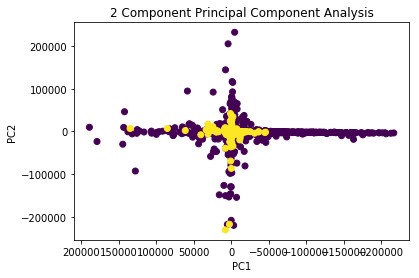
\includegraphics[width=0.6\textwidth]{graphics/pca2.png}
    \caption[Short Caption]{Dimensionality reduction of the data for Year 1 through PCA.}        
    \label{fig:pca}
\end{figure}


\subsection{Experiments} \label{Experiments}

A number of experiments were carried out using the implemented models in order to determine the effects of the various techniques on the model performance. To do so, a baseline for both logistic regression and bagged decision trees were established, and the AUC, sensitivity and specificity were measured using 10-fold cross-validation. The AUC and 10-fold cross-validation were selected based on the arguments brought up by a similar study \cite{zikeba2016ensemble} on the evaluation of classification based on imbalanced data. We also add sensitivity and specificity as a measure of the correctness of the classification. \medskip

Throughout each experiment only one technique is varied from the baseline so that the effect of the change can be quantified. Once again the performance is measured using 10-fold cross-validation. \medskip

As a baseline model for logistic regression, a pipeline incorporating class-partitioned mean imputation and quantile normalisation is taken. Class imbalance is addressed through the use of class weights in the model, that is by giving higher weights to the minority class (bankrupt).\medskip

The baseline model for bagged decision trees incorporates class-partitioned mean imputation and caters for class imbalance through class weights.

Prior to running the experiments, the optimal hyper parameters for each year of the data for both logistic regression and bagged decision trees where searched. Then these were kept constant through all runs of the models. The hyper parameters that were used throughout the experiments are presented in Table~\ref{tab:hyperparam}.

\begin{table}[]
\begin{tabular}{crr|rrr}
\toprule
\multicolumn{1}{l}{\textbf{}} & \multicolumn{2}{c|}{\textbf{Logistic Regression}} & \multicolumn{3}{c}{\textbf{Bagged Decision Trees}} \\
\textbf{Year} & \multicolumn{1}{c}{\textbf{Learning Rate}} & \multicolumn{1}{c}{\textbf{Minimum Loss}} & \multicolumn{1}{c}{\textbf{Max Features (\%)}} & \multicolumn{1}{c}{\textbf{Max Samples (\%)}} & \multicolumn{1}{c}{\textbf{\# Models}} \\
\midrule
\textbf{1} & 0.010 & 0.010 & 0.9 & 0.9 & 11 \\
\textbf{2} & 0.001 & 0.001 & 0.9 & 0.7 & 11 \\
\textbf{3} & 0.010 & 0.010 & 1.0 & 0.8 & 10 \\
\textbf{4} & 0.010 & 0.010 & 0.9 & 0.9 & 11 \\
\textbf{5} & 0.010 & 0.010 & 0.9 & 0.9 & 11 \\
\bottomrule
\end{tabular}
\caption{The hyper parameters that were used throughout the experiments.}
\label{tab:hyperparam}
\end{table}



\subsubsection{Experiment 1 - Measuring the performance when handling class imbalance}

\textit{Setup -} Two imbalance handling techniques are introduced in separate runs of pre-processing-training-testing pipelines. In the first pipeline for each classifier, the SMOTE sampling method is used while in the second pipeline random under-sampling is used. The cross-validated results are then compared against the respective baseline model of the classifier.
\smallskip

\textit{Expected result -} Given the class imbalance in the dataset, performance improvement is expected both over- and under-sampling techniques.
\smallskip

\textit{Actual result -} As seen in Table \ref{tab:lr1}, both SMOTE and random under-sampling  improve the sensitivity but decrease the specificity. This results in a slightly better AUC for SMOTE, but a decreased AUC for random under-sampling for logistic regression. The AUC for bagged decision trees improves marginally with both sampling techniques. Overall, the results show little improvement on the class weights methods embedded into the baseline models.

\begin{table}[ht!]
\begin{tabular}{lrrr|rrr}
\toprule
 & \multicolumn{3}{c|}{\textbf{Logistic Regression}} & \multicolumn{3}{c}{\textbf{Bagged Decision Trees}} \\
 & \textbf{Baseline} & \textbf{SMOTE} & \begin{tabular}[c]{@{}r@{}}\textbf{Random}\\ \textbf{Under-sampling}\end{tabular} & \textbf{Baseline} & \textbf{SMOTE} & \begin{tabular}[c]{@{}r@{}}\textbf{Random}\\ \textbf{Under-sampling}\end{tabular} \\
\midrule
\textit{AUC} & 0.875 & 0.879 & 0.867 & 0.909 & 0.918 & 0.915 \\
\textit{sensitivity} & 0.725 & 0.775 & 0.758 & 0.581 & 0.612 & 0.801 \\
\textit{specificity} & 0.869 & 0.845 & 0.826 & 0.997 & 0.991 & 0.858 \\
\bottomrule
\end{tabular}
\caption{The results for Experiment 1}
\label{tab:lr1}
\end{table}

\subsubsection{Experiment 2 - Measuring the effects of different normalisation techniques on logistic regression}

\textit{Setup -} Three different pipelines are run, each with a different normalisation technique. The quantile normalization in the baseline model is replaced with \textit{min-max} normalisation, \textit{l2} normalisation and \textit{z-score} normalisation.  The cross-validated results are then compared against the baseline, which uses quantile normalisation. This experiment was only run on logistic regression since in the case of bagged decision trees normalisation does not make much sense.
\smallskip

\textit{Expected result -} The baseline model is expected to outperform the other models because the quantile normalisation technique is more robust to outliers, which characterise the dataset being used.
\smallskip

\textit{Actual result -} As it can be seen in Table \ref{tab:lr2}, the normalisation methods under test do not improve on the baseline. Contrarily, the performance is considerably degraded. Figure~\ref{fig:cm_norm} shows the the resulting confusion matrices of the four methods. The considerable decrease in true positives for min-max normalisation (Figure~\ref{fig:cm_norm}b) can be observed, as well as the decrease in true negatives and increase in false positives for l2 normalisation (Figure~\ref{fig:cm_norm}c). Quantile normalisation (Figure~\ref{fig:cm_norm}a) outperforms the other methods possibly due to its resistance to outliers.

\begin{table}[ht!]
\centering
\begin{tabular}{lrrrr}
\toprule
{} & \textbf{Baseline} & \textbf{min-max} & \textbf{l2} & \textbf{z-score} \\
\midrule
\textit{AUC} & 0.875 & 0.513 & 0.697 & 0.751\\
\textit{sensitivity} & 0.725 & 0.672 & 0.545 & 0.661\\
\textit{specificity} & 0.869 & 0.337 & 0.738 & 0.75\\
\bottomrule
\end{tabular}
\caption{The results for Experiment 2}
\label{tab:lr2}
\end{table}

\begin{figure}[ht!]
\centering
\subfloat[Quantile normalisation]{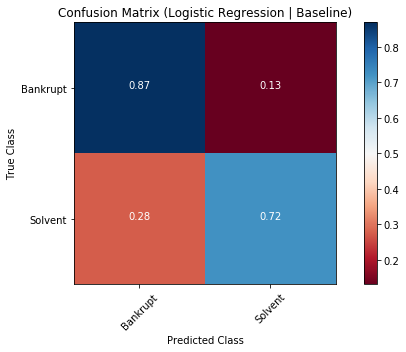
\includegraphics[width=0.45\textwidth]{graphics/cm_lg_base.png}}\qquad
\subfloat[Min-max normalisation]{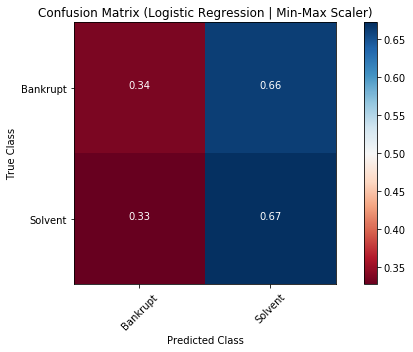
\includegraphics[width=0.45\textwidth]{graphics/cm_lg_minmax.png}}\qquad
\subfloat[L2 normalisation]{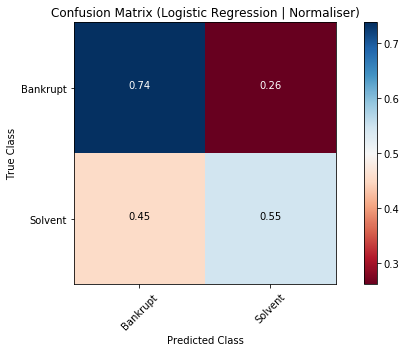
\includegraphics[width=0.45\textwidth]{graphics/cm_lg_l2.png}}\qquad
\subfloat[Z-score normalisation]{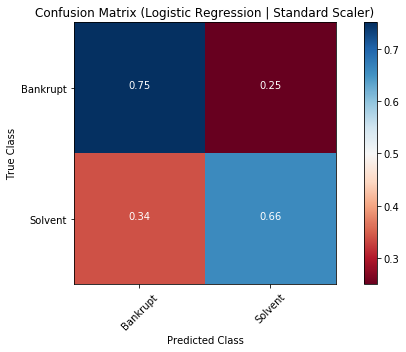
\includegraphics[width=0.45\textwidth]{graphics/cm_lg_zscore.png}}
\caption{The resulting confusion matrices of the different normalisation methods.}
\label{fig:cm_norm}
\end{figure}

\subsubsection{Experiment 3 - Measuring the effects of different feature selection/dimensionality reduction techniques}

\textit{Setup -} In this experiment three pipelines are run for logistic regression and two for bagged decision trees, each adding a feature selection or dimensionality reduction method to the baseline model. The methods under test for logistic regression are PCA, L2 regularisation and k-best features. For bagged decision trees only PCA and k-best features are tested since L2 regularisation does not apply for bagged decision trees. The cross-validated results are then compared to the baseline.
\smallskip

\textit{Expected result -} Due to the correlation observed between some attributes, it is expected that feature selection and dimensionality reduction techniques should improve the performance of the models.
\smallskip

\textit{Actual result -} Although PCA did slightly better than the baseline in terms of AUC for logistic regression, the expected improvement was not observed. In fact, the baseline model performed better than the models having l2 regularisation and k-best features. A slight improvement by PCA was also noted in sensitivity. For bagged decision trees on the other hand, PCA degraded the performance with lower results on all counts. Bagged decision trees with k-best features performed marginally worse than the baseline. This shows that bagged decision trees performs better with high-dimensional data. The results of the experiment can be seen in Table \ref{tab:lr3}.


\begin{table}[ht!]
\begin{tabular}{lrrrr|rrr}
\toprule
 & \multicolumn{4}{c|}{\textbf{Logistic Regression}} & \multicolumn{3}{c}{\textbf{Bagged Decision Trees}} \\
 & \textbf{Baseline} & \textbf{PCA} & \textbf{l2} & \textbf{k-best} & \textbf{Baseline} & \textbf{PCA} & \textbf{k-best} \\
\midrule
\textit{AUC} & 0.875 & 0.877 & 0.874 & 0.865 & 0.909 & 0.875 & 0.902 \\
\textit{sensitivity} & 0.725 & 0.775 & 0.725 & 0.706 & 0.581 & 0.352 & 0.553 \\
\textit{specificity} & 0.869 & 0.839 & 0.87 & 0.866 & 0.997 & 0.996 & 0.997 \\
\bottomrule
\end{tabular}
\caption{The results for Experiment 3}
\label{tab:lr3}
\end{table}

\subsubsection{Experiment 4 - Measuring the effects of different imputation methods on logistic regression}

\textit{Setup -} In this experiment the class-partitioned mean imputation method used in the baseline model is replaced with three other imputation methods. The first method imputes all missing values within an attribute to the mean for the attribute, the second method imputes to the median whilst the third imputes to the of the attribute partitioned by class. The three imputation methods were run for both logistic regression and bagged decision trees. Once again the cross-validated results are then compared to the baseline.
\smallskip

\textit{Expected result -} The baseline already incorporates a strong imputation strategy, which also takes into account the class. So the imputations using the mean and median are not expected to improve the results. The class-partitioned median may slightly improve the results, particularly due to the presence of outliers.
\smallskip

\textit{Actual result -} As seen in Table \ref{tab:lr4}, no improvement in terms of AUC was observed by either of the imputation methods under test for both logistic regression and bagged decision trees. However, the class-partitioned median imputation resulted in a better sensitivity for logistic regression. This cannot be said for bagged decision trees, however, it is noticed that specificity remained stable for all imputation methods.

\begin{table}[ht!]
\begin{tabular}{lrrrr|rrrr}
\toprule
 & \multicolumn{4}{c|}{\textbf{Logistic Regression}} & \multicolumn{4}{c}{\textbf{Bagged Decision Trees}} \\
 & \textbf{Baseline} & \textbf{mean} & \textbf{median} & \textbf{\begin{tabular}[c]{@{}r@{}}class-\\ partitioned\\ median\end{tabular}} & \textbf{Baseline} & \textbf{mean} & \textbf{median} & \textbf{\begin{tabular}[c]{@{}r@{}}class-\\ partitioned\\ median\end{tabular}} \\
\midrule
\textit{AUC} & 0.875 & 0.867 & 0.815 & 0.833 & 0.909 & 0.858 & 0.837 & 0.904 \\
\textit{sensitivity} & 0.725 & 0.725 & 0.73 & 0.742 & 0.581 & 0.385 & 0.301 & 0.517 \\
\textit{specificity} & 0.869 & 0.831 & 0.754 & 0.791 & 0.997 & 0.997 & 0.997 & 0.998 \\
\bottomrule
\end{tabular}
\caption{The results for Experiment 4}
\label{tab:lr4}
\end{table}



\subsection{Models implementation} \label{Models implementation}

The classifiers were evaluated by selecting the model with the highest \textit{ROC AUC} score using stratified k-fold cross-validation. The custom implementation inherits from a base class\footnote{https://scikit-learn.org/stable/modules/generated/sklearn.base.BaseEstimator.html} provided by the reference implementation which permits the usage of a common algorithm for transforming the data (e.g. by scaling) and evaluating the best model (Algorithm \ref{alg:custom_vs_lib}).\medskip

\begin{algorithm}[]
 \KwData{Raw dataset}
 \KwResult{Performance metrics}
 $\textrm{result} \gets \{\}$\;
 \For{$\textrm{Year}$ \textbf{in} $\textrm{Dataset}$}{
   $\{X_{\textrm{train}},y_{\textrm{train}},X_{\textrm{test}},y_{\textrm{test}}\} \gets train\_test\_split(\textrm{Year})$\;
   \For{$\textrm{Classifier}$ \textbf{in} $\textrm{Classifiers}$}{
     $\textrm{pipeline} \gets make\_pipeline(\textrm{Transformer}, \textrm{Classifier})$\;
     $\textrm{model} \gets cross\_validate(\textrm{pipeline}, X_{\textrm{train}},y_{\textrm{train}})$\;
     $\hat{y} \gets predict(\textrm{model}, X_{\textrm{test}})$\;
     $\textrm{performance} \gets evaluate(y_{\textrm{test}}, \hat{y})$\;
     $\textrm{result} \gets \textrm{result} \cup \textrm{performance}$\;
   }
 }
 \caption{Selecting and evaluating the best model.}
 \label{alg:custom_vs_lib}
\end{algorithm}\smallskip

All classifiers implement methods for fitting a model, predicting the class $y$ of the test set $X$, and predicting the probability that $X$ belongs to the true or negative class.

\subsubsection{Logistic Regression} \label{Logistic Regression}

The fitting method initialises the coefficients $\beta$ to 0 and addresses class imbalance by finding the weights $\gamma$ inversely proportional to the class frequencies. The optimal coefficients are then identified using stochastic gradient descent until the maximum number of epochs is reached or the model converges (Algorithm \ref{alg:logit_fit}).\medskip

The probability prediction method uses the coefficients learned from the fitting method to find the probability that each sample in the testing set $X$ belongs to class 1 (bankrupt), and then computes the complement (Equation \ref{eq:negprob}) to find the probability that they belong to class 0 (solvent).\medskip

\begin{equation}\label{eq:negprob}
	Pr(\textrm{Solvent}) = 1 - Pr(\textrm{Bankrupt})
\end{equation}\smallskip

The prediction method predicts the labels $\hat{y}$ of the corresponding testing set $X$ by calling the probability prediction method to apply label 1 to those samples having a probability greater than 0.5 of belonging to class 1, and apply label 0 to those samples which fall below this probability threshold.\medskip

\begin{algorithm}[]
 \KwData{$X_{m \times n},y_{m \times 1},\alpha,\epsilon$}
 \caption{Logistic regression fitting method taking learning rate $\alpha$, stopping criterion $\epsilon$, $m \times n$ training matrix $X$ and corresponding label vector $y$. The logistic function is represented by $\sigma()$.}
 $\beta \gets [0_1,...,0_n]$\;
 $\gamma \gets [1_1,...,1_m]$\;
 \For {$i=0$ \textbf{to} $m$}{
   $\gamma[i] \gets m \times (2 \times |y = y[i]|)^{-1}$\;
 }
 \For{$\textrm{epoch}$ \textbf{in} $\textrm{epochs}$}{
   $\hat{y} \gets \sigma(X \cdot \beta^T)$\;
   $\textrm{loss} \gets cost(y, \hat{y})$\;
   \If{$\textrm{early\_stop}(\textrm{loss}, \epsilon)$}{
     break\;
   }
   $\Delta \gets \frac{1}{m} \times X^T \cdot ((\hat{y} - y) \times \gamma)$\;
   $\beta \gets \beta - (\alpha \cdot \Delta)$\;
 }
 \label{alg:logit_fit}
\end{algorithm}\smallskip

\subsubsection{Decision Tree} \label{imp_decision_tree}

The fitting method calls the build\textunderscore tree method which recursively builds a C4.5 tree (Algorithm \ref{alg:build_tree}). The algorithm creates a multi-way tree, finding for each node in a greedy manner the best\textunderscore split that yields the largest information gain for the categorical targets. The recursion stops when either all nodes are covered or the stop\textunderscore condition is hit. The stop\textunderscore condition depends on the number of samples needed to make the split, minimum information gain and the maximum tree depth.\medskip

Note the custom decision tree implementation, due to all iterations needed for the greedy algorithm runs pretty slow compared to the scikit learn model which is implemented in C. Having said this, to speed-up a bit scipy library\footnote{https://docs.scipy.org/doc/scipy/reference/generated/scipy.stats.entropy.html} is used to calculate the entropy. Note that the raw implementation of entropy is commented out.\medskip

\begin{algorithm}[]
 \KwData{$X,y$}
 \caption{Building a C4.5 Decision Tree from feature set $X$ and label $y$}
 \If{$stop\_condition(X, y)$}{
   return $create\_leaf\_node(y)$\;
 }
 
 $\textrm{impurity}, \textrm{threshold}, \textrm{leftX}, \textrm{rightX}, \textrm{lefty}, \textrm{righty} \gets find\_best\_split({X, y})$\;
 $\textrm{left\_branch} \gets build\_tree(leftX, lefty)$\;
 $\textrm{right\_branch} \gets build\_tree(rightX, righty)$\;
 return $create\_decision\_node(threshold, left\_branch, right\_branch)$\; 
 \label{alg:build_tree}
\end{algorithm}\smallskip


The prediction method does a recursive search down the tree and makes a prediction of the data sample from the outcome value of the ?nal leaf.\medskip

\subsubsection{Bagging} \label{imp_bagging}

The fitting method as shown in (Algorithm \ref{alg:bagging_fit}) trains $n\_e$ number of estimators each time using a sub-feature size $n\_f$ and sub-sample size $n\_s$ randomly picked.\medskip

\begin{algorithm}[]
 \KwData{$X_{m \times n},y_{m \times 1},n\_e,n\_f,n\_s$}
 \caption{Bagging fitting method taking number of estimators $n\_e$, number of sub-feature size $n\_f$, number of sub-sample size $n\_s$, $m \times n$ training matrix $X$ and corresponding label vector $y$}
 \For {$i=0$ \textbf{to} $n\_e$}{
   $X_{n\_s \times n\_f} \gets bootstrap\_feature\_sample(X_{m \times n}, \textrm{n\_f}, \textrm{n\_s})$\;
   $\textrm{estimator} \gets make\_estimator()$\;
   \textrm{estimator.fit}($X_{n\_s \times n\_f}, y_{m \times 1}$)\;
 }
 \label{alg:bagging_fit}
\end{algorithm}\smallskip

The predication method calls each estimator predication method based on the features that the estimator was trained on and then returns the average predictive result.

\subsection{Comparison with third party libraries} \label{Comparison with third party libraries}

The performance of the models developed in this assignment was benchmarked with their counterpart implementations in the \textit{scikit learn\footnote{https://scikit-learn.org}} libraries. The models used for comparison were the \textit{SGDClassifier\footnote{https://scikit-learn.org/stable/modules/generated/sklearn.linear\_model.SGDClassifier.html}} for logistic regression and the \textit{DecisionTreeClassifier\footnote{https://scikit-learn.org/stable/modules/generated/sklearn.tree.DecisionTreeClassifier.html}} and \textit{BaggingClassifier\footnote{https://scikit-learn.org/stable/modules/generated/sklearn.ensemble.BaggingClassifier.html}} for bagged decision trees. The parameters for the models were kept constant.\medskip

Table \ref{tab:sklearn} shows the results of the comparative results of the benchmark test. It can be seen that whilst the scikit learn implementation of logistic regression outperforms our implementation, the performance of our bagged decision trees model is very close to that of scikit learn. It can also be noticed that similar to our implementations,the bagged decision trees model for scikit learn obtained much better results than the logistic regression model. Figure~\ref{fig:sklearn} shows ROC plots for the results. The improved performance of the scikit learn logistic regression model (Figure~\ref{fig:sklearn}b) over its counterpart (Figure~\ref{fig:sklearn}a) can be seen. The similarity between the results of the bagged decision trees models (Figure~\ref{fig:sklearn}c and d) can also be observed. Figure~\ref{fig:cm_sklearn} shows the confusion matrices for the custom models and the \textit{scikit learn} models.

\begin{table}[ht!]
\begin{tabular}{lrr|rr}
\toprule
 & \multicolumn{2}{c|}{\textbf{Logistic Regression}} & \multicolumn{2}{c}{\textbf{Bagged Decision Trees}} \\
 & \textbf{\begin{tabular}[c]{@{}r@{}}custom\\ model\end{tabular}} & \textbf{sk-learn} & \textbf{\begin{tabular}[c]{@{}r@{}}custom\\ model\end{tabular}} & \textbf{sk-learn} \\
\midrule
\textit{AUC} & 0.856 & 0.875 & 0.903 & 0.909 \\
\textit{sensitivity} & 0.749 & 0.725 & 0.636 & 0.581 \\
\textit{specificity} & 0.778 & 0.869 & 0.993 & 0.997 \\
\bottomrule
\end{tabular}
\caption{The results of the benchmark test with \textit{scikit learn} libraries.}
\label{tab:sklearn}
\end{table}

\begin{figure}[!ht]
\centering
\subfloat[Custom logistic regression]{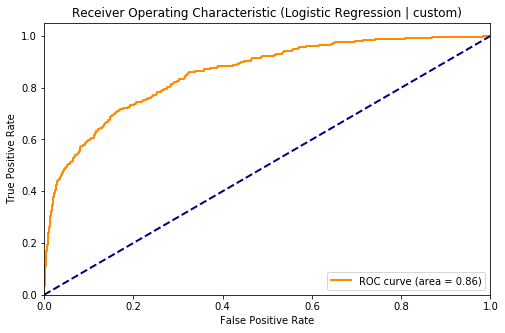
\includegraphics[width=0.45\textwidth]{graphics/roc_lg_custom.png}}\qquad
\subfloat[Scikit learn logistic regression]{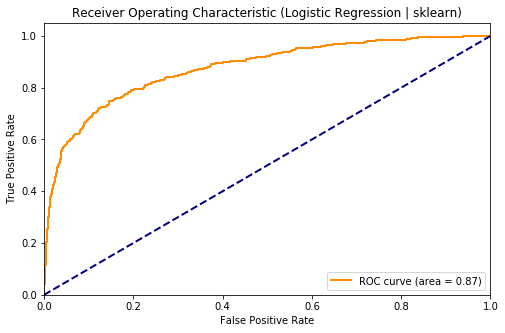
\includegraphics[width=0.45\textwidth]{graphics/roc_lg_sklearn.png}}\qquad
\subfloat[Custom bagged decision trees]{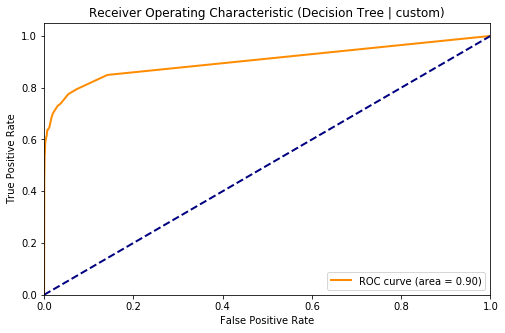
\includegraphics[width=0.45\textwidth]{graphics/roc_dt_custom.png}}\qquad
\subfloat[Scikit learn bagged decision trees]{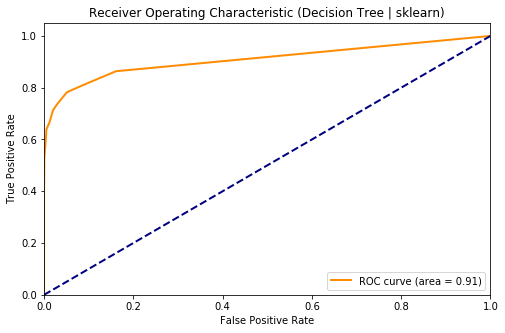
\includegraphics[width=0.45\textwidth]{graphics/roc_dt_sklearn.png}}
\caption{The resulting ROC graphs for the custom implementations and the \textit{scikit learn} implementations of the models.}
\label{fig:sklearn}
\end{figure}

\begin{figure}[ht!]
\centering
\subfloat[Custom logistic regression]{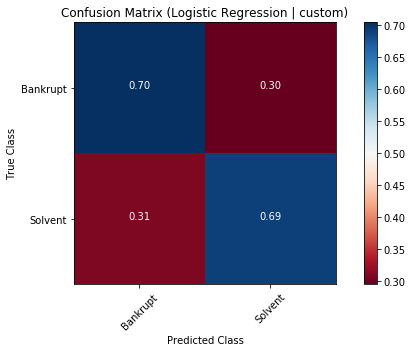
\includegraphics[width=0.45\textwidth]{graphics/cm_lg_base2.png}}\qquad
\subfloat[Scikit learn logistic regression]{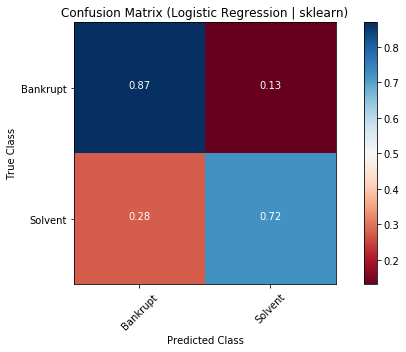
\includegraphics[width=0.45\textwidth]{graphics/cm_lg_sk.png}}\qquad
\subfloat[Custom bagged decision trees]{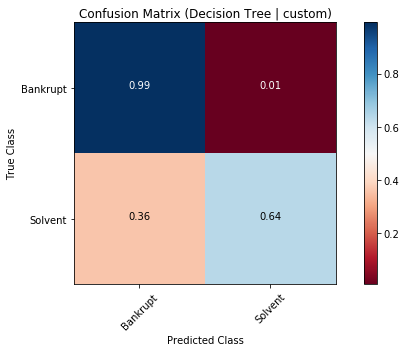
\includegraphics[width=0.45\textwidth]{graphics/cm_dt_base.png}}\qquad
\subfloat[Scikit learn bagged decision trees]{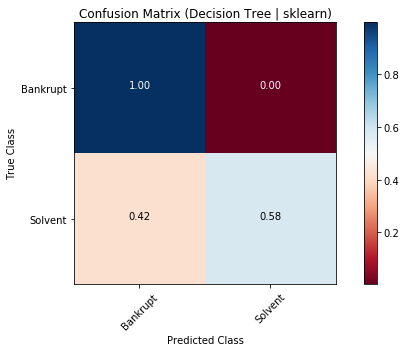
\includegraphics[width=0.45\textwidth]{graphics/cm_dt_sk.png}}
\caption{The resulting confusion matrices for the custom implementations and the \textit{scikit learn} implementations of the models.}
\label{fig:cm_sklearn}
\end{figure}

%----------------------------------------------------------------------------------------
%	CONCLUSION
%----------------------------------------------------------------------------------------

\section{Conclusion}
\label{Conclusion}

In this work we demonstrated that logistic regression and random
forest are suitable machine learning techniques for classifying
instances from the Polish companies dataset as bankrupt or solvent. We
considered various metrics to evaluate the performance. In cases in
which misclassifying bankrupt companies as solvent would incur huge
losses, we recommend that unseen companies are classified with models
that have a higher sensitivity are
preferred over those with higher specificity to minimise the possibility of false
negatives.\medskip

In our experiments we found that bagged decision trees is the best performing
technique that requires little to no preprocessing such as scaling.
It is also robust to outliers and does not benefit from noise
reduction. We found that logistic regression is relatively
straightforward to implement and that it achieves good results by
training a single model rather than an ensemble of weak learners as in
bagged decision trees. Although bagged decision trees were able to classify bankrupt companies much better than logistic regression, they also gave a lot of false positives making them problematic for situations where false positives are costly. \medskip

We also observed an improvement in the performance of
logistic regression when using quantile normalisation since it reduces
the impact of outliers. For both techniques we identified that
class-partitioned mean improved the performance of the models. Moreover, we noticed that class imbalance
is adequately handled by these techniques and extraneous
preprocessing, such as SMOTE or random oversampling, have little to no
effect.\medskip

In future work, we anticipate that further improvements can be
achieved by using coordinate descent to optimise the loss function in
logistic regression since the reference library achieved better results using this technique. Furthermore, we expect that the performance of bagged decision trees can be pushed further
by implementing a boosting technique such as AdaBoost to include in
the ensemble learners with unique classifying characteristics not
found in the other learners.


\bibliographystyle{IEEEtran}
\bibliography{references}

\end{document}
